\documentclass{beamer}
\usepackage[utf8]{inputenc}

\usetheme{Madrid}
\usecolortheme{default}
\usepackage{amsmath,amssymb,amsfonts,amsthm}
\usepackage{txfonts}
\usepackage{tkz-euclide}
\usepackage{listings}
\usepackage{adjustbox}
\usepackage{array}
\usepackage{tabularx}
\usepackage{gvv}
\usepackage{lmodern}
\usepackage{circuitikz}
\usepackage{tikz}
\usepackage{graphicx}
\usepackage{multicol}

\setbeamertemplate{page number in head/foot}[totalframenumber]

\usepackage{tcolorbox}
\tcbuselibrary{minted,breakable,xparse,skins}

\definecolor{bg}{gray}{0.95}
\DeclareTCBListing{mintedbox}{O{}m!O{}}{%
  breakable=true,
  listing engine=minted,
  listing only,
  minted language=#2,
  minted style=default,
  minted options={%
    linenos,
    gobble=0,
    breaklines=true,
    breakafter=,,
    fontsize=\small,
    numbersep=8pt,
    #1},
  boxsep=0pt,
  left skip=0pt,
  right skip=0pt,
  left=25pt,
  right=0pt,
  top=3pt,
  bottom=3pt,
  arc=5pt,
  leftrule=0pt,
  rightrule=0pt,
  bottomrule=2pt,
  toprule=2pt,
  colback=bg,
  colframe=orange!70,
  enhanced,
  overlay={%
    \begin{tcbclipinterior}
    \fill[orange!20!white] (frame.south west) rectangle ([xshift=20pt]frame.north west);
    \end{tcbclipinterior}},
  #3,
}
\lstset{
    language=C,
    basicstyle=\ttfamily\small,
    keywordstyle=\color{blue},
    stringstyle=\color{orange},
    commentstyle=\color{green!60!black},
    numbers=left,
    numberstyle=\tiny\color{gray},
    breaklines=true,
    showstringspaces=false,
}

\title 
{8.3.9}
\date{}

\author
{SAMYAK GONDANE - AI25BTECH11029}

\begin{document}

\frame{\titlepage}

\begin{frame}{Question}
If the latus rectum of an ellipse is equal to half of minor axis, then find its eccentric
\end{frame}

\begin{frame}{Solution}

\textbf{Parametric Vector Form of Ellipse}

An ellipse centered at the origin is defined by the vector function:


\begin{align}
\vec{r}(\theta) =
\myvec{
x(\theta) \\
y(\theta)
}
=
\myvec{
a \cos \theta \\
b \sin \theta
}
\quad \text{where } \theta \in [0, 2\pi]
\end{align}
Here, $a$ and $b$ are the semi-major and semi-minor axes respectively.
\end{frame}



\begin{frame}{Solution}
\textbf{Focus and Latus Rectum}

The focus of the ellipse lies at:


\begin{align}
\vec{F} = 
\myvec{
ae \\
0
}
\quad \text{where } e = \text{eccentricity}
\end{align}


The latus rectum $L$ is the chord perpendicular to the major axis passing through the focus:

\begin{align}
L = \frac{2b^2}{a}
\end{align}
\end{frame}


\begin{frame}{Solution}
\textbf{Given Condition}

We are given:


\begin{align}
L = \frac{1}{2} \cdot 2b = b
\quad \Rightarrow \quad \frac{2b^2}{a} = b
\quad \Rightarrow \quad 2b = a
\end{align}

Thus:

\begin{align}
a = 2b
\end{align}
\end{frame}


\begin{frame}{Solution}
\textbf{Eccentricity via Vector Displacement}

Eccentricity is defined as:


\begin{align}
e = \frac{c}{a}
\quad \text{where } c = \text{distance from center to focus} = \sqrt{a^2 - b^2}
\end{align}

Substitute $a = 2b$:

\begin{align}
c = \sqrt{(2b)^2 - b^2} = \sqrt{4b^2 - b^2} = \sqrt{3b^2} = b\sqrt{3}
\end{align}

\begin{align}
e = \frac{b\sqrt{3}}{2b} = \frac{\sqrt{3}}{2}
\end{align}
\end{frame}


\begin{frame}{Solution}
\textbf{Final Answer}

\begin{align}
\boxed{e = \frac{\sqrt{3}}{2}}
\end{align}
\end{frame}



\begin{frame}{Plot}
    \begin{figure}
        \centering
        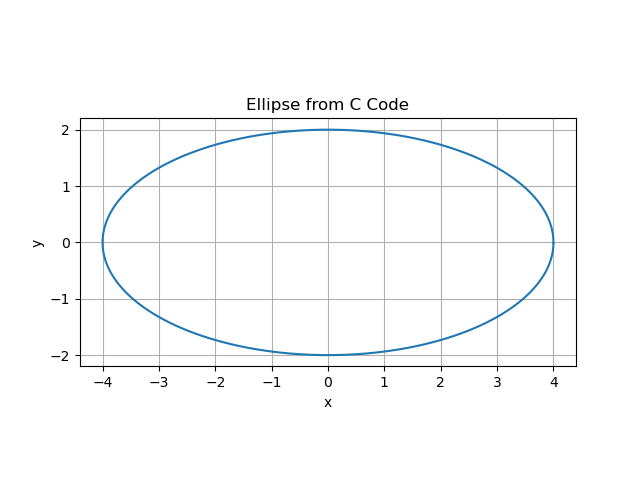
\includegraphics[width=0.7\linewidth]{./figs/Figure_1.png}
        \caption{}
        \label{fig:fig1}
    \end{figure}
\end{frame}

\end{document}